
%(BEGIN_QUESTION)
% Copyright 2006, Tony R. Kuphaldt, released under the Creative Commons Attribution License (v 1.0)
% This means you may do almost anything with this work of mine, so long as you give me proper credit

Bestem en enkel 5-punkts (0\%, 25\%, 50\%, 75\% og 100\%) kalibreringstabell for fortrenger-nivåtransmitteren i dette scenariet:

$$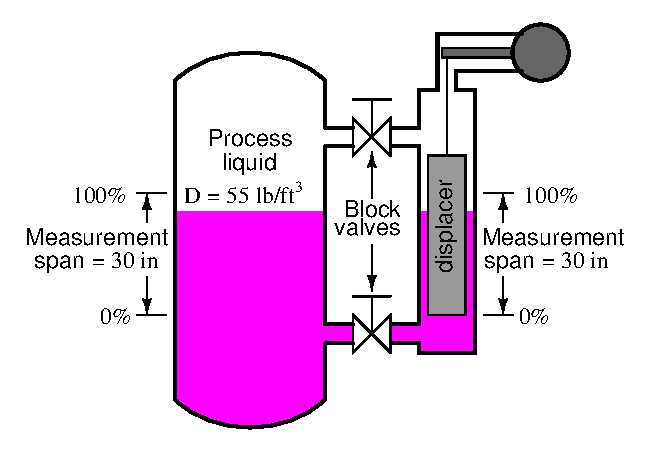
\includegraphics[width=15.5cm]{i00279x01.eps}$$

Den sylindriske fortrengeren veier 15 pund (tørr) og har diameter 3.5 tommer.  Prosessvæsken har tetthet 55 lb/ft$^{3}$.  0\% prosessnivå (LRV) er ved bunnen av fortrengeren.  Anta elektronisk transmittermekanisme med utgangsområde 4 til 20 mA, og kalibreringstoleranse +/- 0.2\% (av spenn).

% No blank lines allowed between lines of an \halign structure!
% I use comments (%) instead, so that TeX doesn't choke.

$$\vbox{\offinterlineskip
\halign{\strut
\vrule \quad\hfil # \ \hfil & 
\vrule \quad\hfil # \ \hfil & 
\vrule \quad\hfil # \ \hfil & 
\vrule \quad\hfil # \ \hfil & 
\vrule \quad\hfil # \ \hfil & 
\vrule \quad\hfil # \ \hfil \vrule \cr
\noalign{\hrule}
%
% First row
Prosess- & Prosent av & Oppdrifts- & Utgangssignal & Utgangssignal & Utgangssignal \cr
%
% Another row
nivå (in) & spenn (\%) & kraft (lb) & ideelt (mA) & min. (mA) & maks. (mA) \cr
%
\noalign{\hrule}
%
% Another row
  & 0 &  &  &  &  \cr
%
\noalign{\hrule}
%
% Another row
  & 25 &  &  &  &  \cr
%
\noalign{\hrule}
%
% Another row
  & 50 &  &  &  &  \cr
%
\noalign{\hrule}
%
% Another row
  & 75 &  &  &  &  \cr
%
\noalign{\hrule}
%
% Another row
  & 100 &  &  &  &  \cr
%
\noalign{\hrule}
} % End of \halign 
}$$ % End of \vbox

\underbar{file i00279}
%(END_QUESTION)





%(BEGIN_ANSWER)

% No blank lines allowed between lines of an \halign structure!
% I use comments (%) instead, so that TeX doesn't choke.

$$\vbox{\offinterlineskip
\halign{\strut
\vrule \quad\hfil # \ \hfil & 
\vrule \quad\hfil # \ \hfil & 
\vrule \quad\hfil # \ \hfil & 
\vrule \quad\hfil # \ \hfil & 
\vrule \quad\hfil # \ \hfil & 
\vrule \quad\hfil # \ \hfil \vrule \cr
\noalign{\hrule}
%
% First row
Prosess- & Prosent av & Oppdrifts- & Utgangssignal & Utgangssignal & Utgangssignal \cr
%
% Another row
nivå (in) & spenn (\%) & kraft (lb) & ideelt (mA) & min. (mA) & maks. (mA) \cr
%
\noalign{\hrule}
%
% Another row
0 & 0 & 0 & 4 & 3.968 & 4.032 \cr
%
\noalign{\hrule}
%
% Another row
7.5 & 25 & 2.297 & 8 & 7.968 & 8.032 \cr
%
\noalign{\hrule}
%
% Another row
15 & 50 & 4.593 & 12 & 11.968 & 12.032 \cr
%
\noalign{\hrule}
%
% Another row
22.5 & 75 & 6.890 & 16 & 15.968 & 16.032 \cr
%
\noalign{\hrule}
%
% Another row
30 & 100 & 9.187 & 20 & 19.968 & 20.032 \cr
%
\noalign{\hrule}
} % End of \halign 
}$$ % End of \vbox

%(END_ANSWER)





%(BEGIN_NOTES)


%INDEX% Calibration: table, level transmitter
%INDEX% Measurement, level: calibration table
%INDEX% Measurement, level: displacer (buoyancy)

%(END_NOTES)
